\documentclass[openbib]{article}

\usepackage{color}
\usepackage{ctex}
\usepackage{mathtools}
\usepackage{amsmath}
\usepackage{graphicx}
% Copyright 20120 Liutao Tian, MIT License
% https://github.com/andy123t/code-latex-style/

\usepackage{listings,color}

% Matlab highlight color settings
%\definecolor{mBasic}{RGB}{248,248,242}       % default
\definecolor{mKeyword}{RGB}{0,0,255}          % bule
\definecolor{mString}{RGB}{160,32,240}        % purple
\definecolor{mComment}{RGB}{34,139,34}        % green
\definecolor{mBackground}{RGB}{245,245,245}   % lightgrey
\definecolor{mNumber}{RGB}{134,145,148}       % gray

\definecolor{Numberbg}{RGB}{237,240,241}     % lightgrey

% Python highlight color settings
%\definecolor{pBasic}{RGB}{248, 248, 242}     % default
\definecolor{pKeyword}{RGB}{228,0,128}        % magenta
\definecolor{pString}{RGB}{148,0,209}         % purple
\definecolor{pComment}{RGB}{117,113,94}       % gray
\definecolor{pIdentifier}{RGB}{166, 226, 46}  %
\definecolor{pBackground}{RGB}{245,245,245}   % lightgrey
\definecolor{pNumber}{RGB}{134,145,148}       % gray

\lstnewenvironment{Python}[1]{
	\lstset{language=python,               % choose the language of the code
		xleftmargin=30pt,
		xrightmargin=10pt,
		frame=l,
		framesep=15pt,%framerule=0pt,  % sets the frame style
		%frame=shadowbox,rulesepcolor=\color{red!20!green!20!blue!20},
		%basicstyle=\small\ttfamily,          % sets font style for the code
		basicstyle=\footnotesize\fontspec{Consolas},
		keywordstyle=\color{pKeyword},       % sets color for keywords
		stringstyle=\color{pString},         % sets color for strings
		commentstyle=\color{pComment},       % sets color for comments
		backgroundcolor=\color{pBackground}, % choose the background color
		title=#1,                            %\lstname show the filename of files
		emph={format_string,eff_ana_bf,permute,eff_ana_btr},
		emphstyle=\color{pIdentifier}
		showspaces=false,                    % show spaces adding particular underscores
		showstringspaces=false,              % underline spaces within strings
		showtabs=false,                      % show tabs within strings adding particular underscores
		tabsize=4,                           % sets default tabsize to 2 spaces
		captionpos=t,                        % sets the caption-position to bottom
		breaklines=true,                     % sets automatic line breaking
		framexleftmargin=5pt,
		fillcolor=\color{Numberbg},
		rulecolor=\color{Numberbg},
		numberstyle=\tiny\color{pNumber},
		numbersep=9pt,                      % how far the line-numbers are from the code
		numbers=left,                        % where to put the line-numbers
		stepnumber=1,                        % the step between two line-numbers.
}}{}

\lstnewenvironment{Python1}[1]{
\lstset{language=python,               % choose the language of the code
  xleftmargin=30pt,
  xrightmargin=10pt,
  frame=l,
  framesep=15pt,%framerule=0pt,  % sets the frame style
  %frame=shadowbox,rulesepcolor=\color{red!20!green!20!blue!20},
  %basicstyle=\small\ttfamily,          % sets font style for the code
  basicstyle=\footnotesize\fontspec{Consolas},
  keywordstyle=\color{pKeyword},       % sets color for keywords
  stringstyle=\color{pString},         % sets color for strings
  commentstyle=\color{pComment},       % sets color for comments
  backgroundcolor=\color{pBackground}, % choose the background color
  title=#1,                            %\lstname show the filename of files
  emph={format_string,eff_ana_bf,permute,eff_ana_btr},
  emphstyle=\color{pIdentifier}
  showspaces=false,                    % show spaces adding particular underscores
  showstringspaces=false,              % underline spaces within strings
  showtabs=false,                      % show tabs within strings adding particular underscores
  tabsize=4,                           % sets default tabsize to 2 spaces
  captionpos=t,                        % sets the caption-position to bottom
  breaklines=true,                     % sets automatic line breaking
  framexleftmargin=5pt,
  fillcolor=\color{Numberbg},
  rulecolor=\color{Numberbg},
  numberstyle=\tiny\color{pNumber},
  numbersep=9pt,                      % how far the line-numbers are from the code
  numbers=left,                        % where to put the line-numbers
  stepnumber=1,                        % the step between two line-numbers.
}}{}



\usepackage{fontspec}
\usepackage{amsfonts}
\graphicspath{{figures/}}
\renewcommand{\contentsname}{\centerline{目录}}

\begin{document}
	\title{数学基础}

	\maketitle
	
	\newpage
	\tableofcontents
	\newpage
\section{数据表示}
	数据表示是机器学习和深度学习的基础,好的数据描述方式对学习算法有促进作用。几乎所有的机器学习和深度学习算法可以看作是张量(Tensor)在各个模块中的流动(Flow)方式。
\subsection{标量,向量,矩阵和张量}
(1)标量(Scalar)

标量其实就是一个只有大小,没有方向独立存在的数,标量的运算相对简单,与数字算术运算类似。

计算机中可以通过一个固定类型的变量来表示。

(2)向量(Vector)

向量是一列数,由一组数组成的有序数组,同时具有大小和方向,通过次序中的索引,我们可以确定每个单独的数。

\[\begin{bmatrix}
	x_1 \\x_2  \\x_3 
\end{bmatrix}\]

向量看作相应线性空间中的一个点,向量中的不同数字还可以用于表示不同坐标轴上的坐标值,向量的方向为原点指向当前空间坐标的方向,向量的大小由范数决定

计算机中通过一个固定长度,固定类型的数组表示,数组的长度就是向量的维数。

(3)矩阵(Matrix)

矩阵就是一个二维数组结构,其中的每一个元素被两个索引所确定,矩阵的索引值是二维的,所以在确定矩阵中的每个元素的位置时需要两个数字。

\[\begin{bmatrix}
	x_{11} & x_{12} \\x_{21} & x_{22}  \\x_{31}& x_{32} 
\end{bmatrix}\]

在计算机中,矩阵可以通过一个固定大小,固定类型的二维数组表示,两个维度分别表示行和列。

(4)张量(Tensor)

若数组的维度超过了二维,就需要使用张量来表示,也可以理解为高维数组,索引值也会跟着产生变化。一般来说,如果一个数组中的元素分布在若干维坐标的规则网格中,我们就称其为张量。

在计算机中,张量可以通过任意维度的数组表示。

\subsection{向量的范数}
向量既有大小又有方向,向量的大小由范数(Norm)来衡量。范数就是衡量从原点到点\textbf{v}的距离。对于一个n维向量$\textbf{v}=(v_1,v_2,v_3,...,v_n)$,形式上,$L_p$范数函数定义为:
$$L_p(\textbf{v})\equiv\left\| \textbf{v} \right\|_p = (\sum_{i=1}^{n}|v_i|^p)^{\frac{1}{p}} \qquad (p\in R \text{且} p\ge1)$$

常用的有L1范数和L2范数。常用的向量的范数如下:

L0范数:$\left\| x \right\|$0为x向量各个非零元素的个数。

L1范数(Lasso Regularization 稀疏规则算子):$\left\| x \right\|$1为x向量各个元素绝对值之和。当p等于1时即为$L_1$范数,通常$L_1$范数用于区分零元素和非零但值很小的元素。例如在损失函数正则化项的计算中,选择$L_1$范数。

L2范数(Euclidean范数或Frobenius范数):$\left\| x \right\|$2为x向量各个元素平方和的1/2次方。当p等于2时,$L_2$范数称为欧几里得范数(Euclidean Norm)或(Frobenius 范数),它表示从原点出发到向量\textbf{v}的欧几里得距离。运用广泛,经常会写作$||\textbf{v}||$。为了计算方便,使用平方的$L_2$范数,简单的利用点积$\textbf{v}^T\textbf{v}$来计算。常常会省略下标2.

Lp范数:$\left\| x \right\|$为x向量各个元素绝对值p次方和的1/p次方。

L$\infty$范数:$\left\| x \right\|$为x向量各个元素绝对值最大元素的绝对值。

当p趋于$\infty$时为$L_{\infty}$范数即最大范数(max norm)。$L_{\infty}$范数表示向量中最大分量的绝对值:
$$\left\|\textbf{v}\right\|_{\infty} = \underset{i}{max}|v_i|$$
性质:

1.非负性:范数函数的值永远非负,当且仅当向量为全零向量时,范数函数值为0。
\begin{equation*}
	\begin{aligned}
f(\textbf{x})\ge0	\\
f(\textbf{x})=0\Rightarrow \textbf{x}=\textbf{0}
	\end{aligned}
\end{equation*}

2.三角不等式:两个向量范数的和大于两个向量和的范数。
$$f(\textbf{x})+f(\textbf{y})\ge f(\textbf{x}+\textbf{y})$$

3.正值齐次性:
$$\forall a\in R, \qquad f(a\textbf x) = \left| a \right|f(\textbf x)$$

\subsection{常用的向量}
\textbf{全0向量}指所有分量都为0的向量。
$$\textbf{0}= \begin{aligned}
	\begin{bmatrix}
		0 \\0  \\ \vdots \\ 0
	\end{bmatrix}
\end{aligned}$$ 

\textbf{全1向量}指所有分量都为1的向量。
$$\textbf{1}= \begin{aligned}
	\begin{bmatrix}
		1 \\1  \\ \vdots \\ 1
	\end{bmatrix}
\end{aligned}$$ 

\textbf{One-Hot向量}指有且仅有一个分量为1,其他分量为0的向量。One-Hot向量属于稀疏的编码,默认不同的分量之间是没有关联的,广泛运用于编码中。

物体分类应用中,我们通常将分类的结果编码为一个One-Hot向量,元素为1的那个分类对应的类别为分类得到的类别。

自然语言处理应用中,也会使用One-Hot向量为每一个词编码再进行处理。

\textbf{单位向量}(unit vector)即单位向量的$L_2$范数为1,单位向量约束了向量的长度为1,屏蔽向量模长带来的影响。只能表达该向量的方向,向量方向的性质。

余弦相似性(cosine similarity)比较两个向量的夹角,从而考虑两个向量的相关性。
$$cos\theta = \textbf{u}^T\textbf{v}=\textbf{v}^T\textbf{u}$$
其中,$\theta$为两个向量的夹角,\textbf{u}和\textbf{v}为两个单位向量。

\subsection{常见矩阵}
\textbf{方阵}:指行数等于列数的矩阵。
$$\textbf{A}_{m\times n}, m=n$$
\textbf{对称矩阵(symmetric matrix)}:指它的转置就等于它本身的矩阵。列如无向图的顶点邻接矩阵。
$$\textbf{A}^T = \textbf{A}$$
\textbf{对角矩阵(diagonal matrix)}:指只在主对角线上含有非零元素,其他元素都为0的矩阵。单位矩阵是一种特殊的对角矩阵。
$$a_{ij}=0,i\neq j$$
\textbf{正定矩阵(positive definite matrix)}:方阵textbf{M}是正定矩阵的充要条件:顺序主子式的行列式都大于0;矩阵特征值都大于0。

对于任意的非零向量z。都有$$z^T\textbf{M}z>0$$
\textbf{半正定矩阵(positive semidefinite matrix)}:方阵\textbf{M}是半正定矩阵的充要条件是:顺序主子式的行列式都非负;矩阵特征值都非负。

对于任意的非零向量z,都有$$z^T\textbf{M}z\ge0$$
\textbf{负定矩阵(negative definite matrix)}:方阵\textbf{M}是负定矩阵的充要条件是:第奇数个顺序主子式的行列式都小于0,第偶数个顺序主子式的行列式都大于0;矩阵特征值都小于0。

对于任意的非零向量z,都有$$z^T\textbf{M}z<0$$
\textbf{正交矩阵(orthogonal matrix)}:逆矩阵等于它的转置矩阵的方阵。正交矩阵的行向量和列向量分别都是标准正交的
$$A^{T}=A^{-1}$$
当其范数为1时,我们称它们是标准正交(orthonormal)
\subsection{矩阵的操作}
\textbf{矩阵的转置(transpose)}:矩阵的转置就是以主对角线为轴的镜像矩阵,这条从左上角到右下角的对角线被称为主对角线(main diagonal)
$$[\textbf{A}^T]_{ij}=[\textbf{A}]_{ji}$$
标量可以看作是只有一个元素的矩阵。因此,标量的转置等于它本身
\\textbf{矩阵的Frobenius范数(Frobenius Norm)}:衡量矩阵的大小。矩阵$\textbf{A}=(a_{ij})$的Frobenius范数为
$$\left\| \textbf{A} \right\|_{F}=\sqrt{\sum_{i,j}^{}a_{ij}^2}$$
\textbf{矩阵与矩阵相加}:只要矩阵的形状一样,我们可以把两个矩阵相加,设矩阵$\textbf{A}=(a_{ij})$和$\textbf{B}=(b_{ij})$是$m\times n$的矩阵,那么两矩阵相加也是$m\times n$的矩阵,其中每个元素都是\textbf{A}和\textbf{B}的对应元素相加
$$[\textbf{A}+\textbf{B}]_{ij}=a_{ij}+b_{ij}$$
\textbf{矩阵与向量相加}:在数学上矩阵和向量无法相加,但在深度学习中允许。具体过程就是使向量与矩阵中的所有列向量分别相加。设$\textbf{A}=(a_{ij})$是$m\times n$矩阵,$\textbf{b}=(b_i)$是m维向量,则$\textbf{A}+\textbf{b}$的第i行第j列元素为:
$$[\textbf{A}+\textbf{b}]_{ij}=\textbf{A}_{ij}+b_{ij}$$

广播(broadcasting):隐式复制向量到很多位置参与计算,能够提升编码的效率和运行效率。
\\\textbf{矩阵与标量相加}:矩阵$\textbf{A}=(a_{ij})$与标量b相加,就将标量和矩阵的所有的元素相加。
$$[\textbf{A}+b]_{ij}=\textbf{A}_{ij}+b$$
\textbf{矩阵与矩阵相乘}:第一个矩阵的列数需要等于第二个矩阵的行数。如果$\textbf{A}=(a_{ij})$是$k\times m$矩阵和$\textbf{B}=(b_{ij})$是$m\times n$矩阵,则乘积\textbf{AB}是一个$k\times n$的矩阵。
$$[\textbf{AB}]_{ij}=\sum_{k=1}^{m}a_{ik}b_{kj}$$
矩阵乘法服从分配律和结合律,不服从交换率。矩阵乘积的转置等于矩阵转置的倒序乘积。
\\\textbf{矩阵与向量相乘}:可看成矩阵与一列矩阵相乘。设$\textbf{A}=(a_{ij})$是$m\times n$矩阵和$\textbf{b}=(b_{i})$是m维向量,则乘积\textbf{Ab}是一个m维向量。
$$[\textbf{Ab}]_{i}=\sum_{k=1}^{m}a_{ik}b_{k}$$
\textbf{矩阵与标量相乘}:矩阵$\textbf{A}=(a_{ij})$与标量b相乘就是将标量与矩阵的每个元素相乘。
$$[b\textbf{A}]_{ij}=a_{ij}b$$
\textbf{矩阵的行列式(determinant)}:一个方阵的行列式等于任意一行或一列上所有元素$a_{ij}$与其对应代数余子式$(-1)^{i+j}\textbf{M}_{ij}$乘积的和。
$$det(\textbf{A})=\sum_{j=1}^{n}a_{ij}(-1)^{ij}\textbf{M}_{ij}$$
\textbf{矩阵的逆(inversion)}:设\textbf{A}是一个矩阵,如果矩阵\textbf{B}满足$\textbf{AB}=\textbf{BA}=\textbf{I}$,则称\textbf{B}是\textbf{A}的逆矩阵,记为$A^{-1}$。只有行列式不为0的方阵才存在对应的逆矩阵
\\\textbf{矩阵的迹(trace)}:一个方阵$\textbf{A}=(a_{ij})$的迹等于它主对角线上的所有元素的求和。
$$tr(\textbf{A})=\sum_{i=1}^{n}a_{ij}$$
例如矩阵的Frobenius范数可以利用迹
$$\left\| \textbf{A} \right\|_{F}=\sqrt{tr(\textbf{A}\textbf{A}^T)}$$
\textbf{特征分解(eigen decomposition)}:一个方阵分解为一组\textbf{特征值(eigenvalue)}和对应的一组\textbf{特征向量(eigenvector)}。如果一个n阶方阶和一个n维向量\textbf{v}及标量$\lambda$之间有如下关系:$$\textbf{Av}=\lambda\textbf{v}$$
则向量\textbf{v}称为矩阵\textbf{A}的特征向量,标量$\lambda$称为矩阵\textbf{A}的特征值。一个n阶方阵一般有n个特征值$\lambda_1,\lambda_2,...,\lambda_n$,对应的有n个对应特征向量$\textbf{v}^{*(1)},\textbf{v}^{(2)},...,\textbf{v}^{(n)}$

当矩阵$\textbf{v}$可逆时,\textbf{A}可分解为:$$\textbf{A}=\textbf{V}diag(\lambda)\textbf{V}^{-1}$$
其中$diag(\lambda)$表示以$\lambda_1,\lambda_2,...,\lambda_n$,为对角线元素的对角矩阵。特征分解可能并不唯一。

所有特征值都是正数的矩阵被称为 正定(positive definite);所有特征值都是非负数的矩阵被称为 半正定(positive semidefinite)。同样地,所有特征值都是负数的矩阵被称为 负定(negative definite);所有特征值都是非正数的矩阵被称为 半负定
(negative semidefinite)。
\\\textbf{奇异值分解(singular value decomposition,SVD)}:设$\textbf{A}$是$m\times n$实矩阵,$\textbf{A}^{T}\textbf{A}$的特征值为$\lambda_1\ge\lambda_2\ge...\ge\lambda_r\ge\lambda_{r+1}=...=\lambda_n=0$,则称$\theta_i=\sqrt{\lambda_i}(i=1,2,3,...,n)$为矩阵\textbf{A}的\textbf{奇异值(singular value)}
\\矩阵\textbf{A}的奇异值分解是指$\textbf{A}=\textbf{U}\begin{pmatrix}
	\textbf{D}_r & \textbf{0} \\
	\textbf{0} & \textbf{0}
\end{pmatrix}_{m\times n}\textbf{V}^T$,其中矩阵\textbf{U}是$m\times m$正交矩阵,矩阵\textbf{V}是$n\times n$正交矩阵,\textbf{D}是r阶对角矩阵,其主对角线上的元素是矩阵\textbf{A}的全部非零奇异值。方阵\textbf{U}的列向量被称为左奇异向量,矩阵\textbf{V}的列向量被称为右奇异向量

矩阵\textbf{A}的左奇异向量为$\textbf{A}\textbf{A}^{T}$的特征向量,右奇异向量实际为$\textbf{A}^{T}\textbf{A}$的特征向量。
\\\textbf{Moore-Penrose伪逆}:实际应用中,遇到的是非方阵,其逆矩阵没有定义。比如在求解最小二乘回归问题:$$\textbf{Ax}=\textbf{y}$$其中,如果矩阵\textbf{A}是一个行数大于列数的矩阵,不存在确定解,故引入伪逆解定义式:$$\textbf{A}^+=\lim_{a \to 0^+} (\textbf{A}^T\textbf{A}+a\textbf{I})^{-1}\textbf{A}^T$$
实际求解使用奇异值分解的方法:$$\textbf{A}^+=\textbf{VD}^+\textbf{U}^T$$
其中,矩阵$\textbf{U,D,V}$是矩阵$\textbf{A}$奇异解分解后得到的矩阵。伪逆矩阵$\textbf{D}^+$是矩阵\textbf{D}中非零元素取倒数之后再转置得到的。

当矩阵$\textbf{A}$的列数多于行数时,使用伪逆求解线性方程是众多可能解法中的一种。特别地,$x=\textbf{A}^+y$是方程所有可行解中x的欧几里得范数最小的一个

当矩阵$\textbf{A}$的行数多于列数时,可能没有解。通过伪逆得到的x使得Ax和y的欧几里得距离Ax-y最小
\subsection{主成分分析}
主成分分析(principal components analysis,PCA)是一个简单的机器学习算法,可以通过基础的线性代数知识推导。PCA是找到一个新的坐标系,它的原点落在数据的中心,坐标系的方向是往数据分布的方向走。而我们要存储的信息就是新坐标系的原点和相对原来坐标系旋转的角度,原点一般为数据中心点,坐标系找数据分布最分散的方向(方差最大),作为坐标轴(主成分),最重要的是找旋转的角度

假设在$\mathbb{R}^n$空间中我们有m个点,希望对这些点进行有损压缩。有损压缩表示我们使用更少的内存,但损失一些精度去存储这些点,希望损失的精度尽可能的少。

一种编码这些点的方式是用低维表示。对于每一个$x^{(i)}\in \mathbb{R}^n$,会有一个对应的编码向量$c^{(i)}\in \mathbb{R}^l$.如果l比n小,那么我们便使用了更少的内存来存储原来的数据。编码函数,根据输入返回编码,$f(x)=c$;解码函数,给定编码重构输入,$x\approx g(f(x))$


首先:去中心化(把坐标原点放在数据中心),然后:找坐标系(找到方差最大的方向)。可以转换成求解旋转矩阵R,进而能够求出旋转角度。协方差矩阵的特征向量就是R。

定义一个旋转矩阵R,拉伸矩阵S。原始数据D拉伸之后得到的为D'。
协方差(x,y的平均值都为0):
$$cov(x,y)=\frac{\sum_{i-1}^{n}(x_i-\hat{x}(y_i-\hat{y}))}{n-1}=\frac{\sum_{i=1}^{n}x_iy_i}{n-1}$$
协方差矩阵:
$$c=\begin{bmatrix}
	cov(x,x) &cov(x,y)  \\
	cov(x,y)& cov(y,y)
\end{bmatrix}$$
白数据的协方差矩阵为单位矩阵,x和y是不相关的。
$$c=\begin{bmatrix}
	\frac{\sum_{i=1}^{n}x_i^2}{n-1} &\frac{\sum_{i=1}^{n}x_iy_i}{n-1}  \\
	\frac{\sum_{i=1}^{n}x_iy_i}{n-1}& \frac{\sum_{i=1}^{n}y_i^2}{n-1}
\end{bmatrix}=\frac{1}{n-1}\begin{bmatrix}
x_1 &x_2 &x_3 &x_4 \\
y_1 &y_2 &y_3 &y_4
\end{bmatrix}\begin{bmatrix}
x_1 &y_1 \\
x_2 &y_2 \\
x_3 &y_3 \\
x_4 &y_4
\end{bmatrix}=\frac{1}{n-1}DD^T$$
D-数据

数据的协方差$$
C' = \frac{1}{n-1}D'D^T=\frac{1}{n-1}RSD(RSD)^T=\frac{1}{n-1}RSDD^TS^TR^T=RS(\frac{1}{n-1}DD^T)S^TR^T$$

由于白数据的协方差为单位矩阵,即$\frac{1}{n-1}DD^T=C=I$,拉伸矩阵$S=S^T$,旋转矩阵$R^T=R^{-1}$
故
$$C' = RSS^TR^T=RLR^{-1} \qquad L=SS^T=\begin{bmatrix}
	a^2 & 0 \\
	0 & b^2
\end{bmatrix}$$
a,b为定义拉伸矩阵,在各个方向上的拉伸倍数。而$a^2,b^2$是所要求的轴方向上的方差,同时又是协方差矩阵的特征值。

具体地,为了简化解码器,我们使用矩阵乘法将编码映射回$\mathbb{R}^n$,即$g(c)=Dc$,其中$D\in \mathbb{R}^{n\times l}$是定义解码的矩阵。

目前为止所描述的问题,可能会有多个解。因为如果我们按比例地缩小所有点对应的编码向量$c_i$,那么只需按比例放大$D_{:,i}$,即可保持结果不变。为使问题有唯一解,限制D中所有的列向量都有单位范数。PCA限制D的列向量彼此正交。

首先我们需要明确如何根据每一个输入x得到一个最优编码$c^*$。一种方法是最小化原始输入向量x和重构向量$g(c^*)$之间的距离。我们使用$L^2$范数来衡量它们之间的距离。
$$c^*=\underset{c}{argmin}||x-g(c)||_2$$
我们也可以用平方$L^2$范数代替$L^2$范数。因为两者在相同的值c上取得最小值。这是因为$L^2$范数是非负的,并且平方运算在非负值上是单调递增的。
\begin{equation*}
	\begin{split}
	c^*&=\underset{c}{argmin}||x-g(c)||^2_2=\underset{c}{argmin}x^Tx-2x^Tg(c)+g(c)^Tg(c)\\&=\underset{c}{argmin}-2x^Tg(c)+g(c)^Tg(c)=\underset{c}{argmin}-2x^TDc+c^TD^TDc\\&=\underset{c}{argmin}-2x^TDc+c^TI_lc=\underset{c}{argmin}-2x^TDc+c^Tc
	\end{split}
\end{equation*}
通过向量微积分来求解这个最优化问题:$$\bigtriangledown_c(-2x^TDc+c^Tc)=0\to -2D^Tx+2c=0\to c=D^Tx$$
最优编码x只需要一个矩阵-向量乘法操作。为了编码向量,我们使用编码函数:$f(x)=D^Tx$回代,定义PCA重构操作:
$$r(x)=g(f(x))=DD^Tx$$
\begin{Python}{PCA代码段}
from __future__ import division
import numpy as np
import pandas as pd

# 根据保留多少维特征进行降维
class PCAcomponent(object):
	def __init__(self, X, N=3):
		self.X = X
		self.N = N
		self.variance_ratio = []
		self.low_dataMat = []

	def _fit(self):
		X_mean = np.mean(self.X, axis=0)
		dataMat = self.X - X_mean
		# 另一种计算协方差矩阵的方法:dataMat.T * dataMat / dataMat.shape[0]
		# 若rowvar非0,一列代表一个样本;为0,一行代表一个样本
		covMat = np.cov(dataMat, rowvar=False)
		# 求特征值和特征向量,特征向量是按列放的,即一列代表一个特征向量
		eigVal, eigVect = np.linalg.eig(np.mat(covMat))
		eigValInd = np.argsort(eigVal)
		eigValInd = eigValInd[-1:-(self.N + 1):-1]  # 取前N个较大的特征值
		small_eigVect = eigVect[:, eigValInd]  # *N维投影矩阵
		self.low_dataMat = dataMat * small_eigVect  # 投影变换后的新矩阵
		# reconMat = (low_dataMat * small_eigVect.I) + X_mean  # 重构数据
		# 输出每个维度所占的方差百分比
		[self.variance_ratio.append(eigVal[i] / sum(eigVal)) for i in eigValInd]
		return self.low_dataMat

	def fit(self):
		self._fit()
		return self


# 根据保留多大方差百分比进行降维
class PCApercent(object):
	def __init__(self, X, percentage=0.95):
		self.X = X
		self.percentage = percentage
		self.variance_ratio = []
		self.low_dataMat = []

# 通过方差百分比选取前n个主成份
	def percent2n(self, eigVal):
		sortVal = np.sort(eigVal)[-1::-1]
		percentSum, componentNum = 0, 0
		for i in sortVal:
			percentSum += i
			componentNum += 1
			if percentSum >= sum(sortVal) * self.percentage:
				break
		return componentNum

	def _fit(self):
		X_mean = np.mean(self.X, axis=0)
		dataMat = self.X - X_mean
		covMat = np.cov(dataMat, rowvar=False)
		eigVal, eigVect = np.linalg.eig(np.mat(covMat))
		n = self.percent2n(eigVal)
		eigValInd = np.argsort(eigVal)
		eigValInd = eigValInd[-1:-(n + 1):-1]
		n_eigVect = eigVect[:, eigValInd]
		self.low_dataMat = dataMat * n_eigVect
		[self.variance_ratio.append(eigVal[i] / sum(eigVal)) for i in eigValInd]
		return self.low_dataMat

	def fit(self):
		self._fit()
		return self

df = pd.read_csv(r'iris.txt', header=None)
data, label = df[range(len(df.columns) - 1)], df[[len(df.columns) - 1]]
data = np.mat(data)
print("Original dataset = {}*{}".format(data.shape[0], data.shape[1]))
#pca = PCAcomponent(data, 3)
pca = PCApercent(data, 0.98)
pca.fit()
print(pca.low_dataMat)
print(pca.variance_ratio)
\end{Python}
\subsection{常用函数地有用性质}
\begin{center}
	1.logistic sigmoid函数
\end{center}
$$\xi(x) = \frac{1}{1+exp(-x)}$$
sigmoid函数在变量取绝对值非常大的正值或负值会出现饱和现象,意味着函数会变得很平,并且对输入的微小改变会变得不敏感。
\begin{center}
	2.softpluse函数
\end{center}
$$\xi(x)=log(1+exp(x))$$
softplus 函数可以用来产生正态分布的 $\beta$和 $\sigma$ 参数,因为它的范围是$(0,\infty)$。当处理包含 sigmoid 函数的表达式时它也经常出现。
\subsection{距离公式}
(1)闵可夫斯基距离

闵可夫斯基距离(Minkowski distance)是衡量数值点之间距离的一种常见方法。
\begin{figure}[htbp]
	\centering
	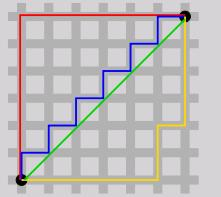
\includegraphics[scale=1]{闵可夫斯基距离.jpg}
	\caption{闵可夫斯基距离}
	\label{a}
\end{figure}

闵可夫斯基距离定义为$\left( \sum_{i=1}^{n}\left| x_{i}-y_{i} \right|^{p} \right)^{1/p}$。最常用的p是2和1。

(2)欧几里得距离(Euclidean distance)

p=2是欧几里得距离,标明两个点在标准坐标系上的直线距离。

例如:二维空间的公式:
$$\rho=\sqrt{(x_{2}- x_{1})^2+(y_{2}-y_{1})^2}$$其中$\rho$为为点$(x_{2},y_{2})$与点$(x_{1},y_{1})$之间的欧氏距离。

三维空间的公式:$$\rho=\sqrt{(x_{2}- x_{1})^2+(y_{2}-y_{1})^2+(z_{2}-z_{1})^2}$$

n维空间的公式:$$\rho=\sqrt{\sum_{i=1}^{n}(x_i-y_i)^2}=\sqrt{(x_{1}- y_{1})^2+(x_{2}-y_{2})^2+...+(x_{n}-y_{n})^2}$$

(3)曼哈顿距离(Manhattan distance)

p=1是曼哈顿距离,标明两个点在标准坐标系上的绝对轴距离总和,在计算距离时不涉及对角线移动。

如上图\ref{a}假设在曼哈顿街区乘坐出租车,白色表示高楼大厦,灰色表示街道。斜线表示欧几里得距离,其他三条表示曼哈顿距离,且三条距离相等。

$$
D(x,y)=\sum_{i=1}^{k}\left| x_i-y_i \right|
$$

(4)切比雪夫距离(Chebyshev distance)

当p趋于无穷大,闵可夫斯基距离转化成切比雪夫距离:
\begin{equation*}
	\lim\limits_{p \to \infty } \left( \sum_{i=1}^{n}\left| x_{i}-y_{i} \right|^{p} \right)^{1/p} = \mathop{max}_{i=1}^n \left| x_{i}-y_{i} \right|
\end{equation*}

向量空间中的一种度量,二个点之间的距离定义是其各坐标数值差绝对值的最大值也就是沿着一个轴的最大距离。切比雪夫距离通常被称为棋盘距离,因为国际象棋的国王从一个方格到另一个方格的最小步数等于切比雪夫距离。

(5)曼哈顿距离与切比雪夫距离的联系

考虑在一个二维坐标系中,设原点为(0,0)如果用曼哈顿距离表示,则与原点距离为1的点会构成一个边长为$\sqrt{2}$的正方形。如图\ref{b}。

\begin{figure}[htbp]
	\centering
	\begin{minipage}[t]{0.48\textwidth}
		\centering
		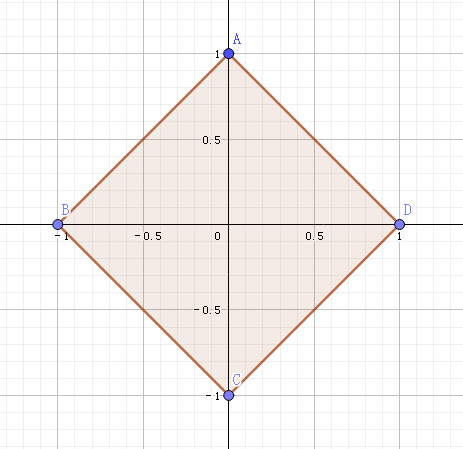
\includegraphics[scale=0.35]{曼哈顿距离.png}
		\caption{曼哈顿距离}
		\label{b}
	\end{minipage}
	\begin{minipage}[t]{0.48\textwidth}
		\centering
		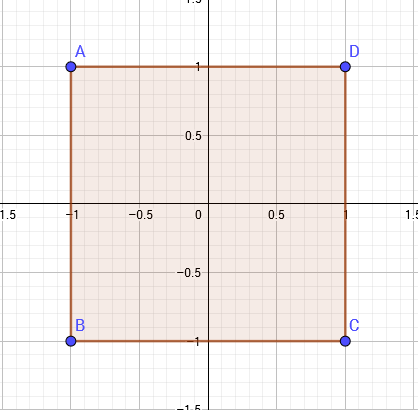
\includegraphics[scale=0.35]{切比雪夫距离.png}
		\caption{切比雪夫距离}
		\label{c}
	\end{minipage}
\end{figure}

如果用切比雪夫距离表示,则与原点距离为1的点会构成一个边长为2的正方形。如图\ref{c}。

因此平面的切比雪夫距离可以视为平面曼哈顿距离旋转再放大后的结果。

事实上,
将一个点(x,y)的坐标变为$(x+y,x−y)$后,原坐标系中的曼哈顿距离 = 新坐标系中的切比雪夫距离

将一个点(x,y)的坐标变为$(\frac{x+y}{2},\frac{x−y}{2})$ 后,原坐标系中的切比雪夫距离 = 新坐标系中的曼哈顿距离

进行推广到高维空间和一点有相等切比雪夫距离的点会形成一个立方体,各面都和坐标轴垂直,而和一点有相等曼哈顿距离的点会形成一个正八面体。

\textcolor{red}{(6)马氏距离(Mahalanobis distance)}

表示数据的协方差距离,有效地计算两个未知样本集地相似度的方法。与欧氏距离不同的是它考虑各种特性之间的联系(列如:一条关于身高的信息会带来一条关于体重的信息。)

对于一个均值为$\mu$,协方差矩阵为$\sum$的多变量向量,其马氏距离为$(x-\mu)'\sum ^{(-1)}(x-\mu)$

马氏与欧式距离的比较:

1)马氏距离的计算是建立在总体样本的基础上的,这一点可以从上述协方差矩阵的解释中可以得出,也就是说,如果拿同样的两个样本,放入两个不同的总体中,最后计算得出的两个样本间的马氏距离通常是不相同的,除非这两个总体的协方差矩阵碰巧相同;

2)在计算马氏距离过程中,要求总体样本数大于样本的维数,否则得到的总体样本协方差矩阵逆矩阵不存在,这种情况下,用欧氏距离计算即可。

3)还有一种情况,满足了条件总体样本数大于样本的维数,但是协方差矩阵的逆矩阵仍然不存在,比如三个样本点(3,4),(5,6)和(7,8),这种情况是因为这三个样本在其所处的二维空间平面内共线。这种情况下,也采用欧氏距离计算。

4)在实际应用中“总体样本数大于样本的维数”这个条件是很容易满足的,而所有样本点出现3)中所描述的情况是很少出现的,所以在绝大多数情况下,马氏距离是可以顺利计算的,但是马氏距离的计算是不稳定的,不稳定的来源是协方差矩阵,这也是马氏距离与欧氏距离的最大差异之处。

优点:它不受量纲的影响,两点之间的马氏距离与原始数据的测量单位无关,由标准化数据和中心化数据(即原始数据与均值之差)计算出的二点之间的马氏距离相同。马氏距离还可以排除变量之间的相关性的干扰。

缺点:它的缺点是夸大了变化微小的变量的作用。

(7)余弦相似度(余弦相似性)

通过计算两个向量的夹角余弦值来评估它们的相似度。

假设向量a,b的坐标分别为$(x_1,y_1)$,$(x_2,y_2)$。则

$$cos\theta = \frac{a\bullet b}{\left\| a \right\|\left\| b \right\|}$$

设向量$\overrightarrow{A}=\left( A_1,A_2,\cdots ,A_n \right)$,$\overrightarrow{B}=\left( B_1,B_2,\cdots ,B_n \right)$。

推广到多维:

\begin{align*}
	cos\theta &= \frac{x_1x_2+y_1y_2}{\sqrt{x_1^2+y_1^2}\times \sqrt{x_2^2+y_2^2}} & 
	cos\theta &= \frac{\sum_{1}^{n}(A_{i}\times B_{i})}{\sqrt{\sum_{1}^{n}A_{i}^2}\times \sqrt{\sum_{1}^{n}B_{i}^2}}
\end{align*}

余弦值的范围在[-1,1]之间,值越趋于1,代表两个向量的方向越趋于0,它们的方向更加一致,相似度也越高。

(8)正则化

为了防止过拟合现象,我们加入正则化项或采用Dropout方法

\begin{center}
	\textcolor{red}{a.加入正则化项}
\end{center}


\subsection{张量的常用操作}
有些常用操作:\textbf{索引(indexing),切片(slicing),连接(joining),换位(mutating)}

\textbf{换位}:矩阵的转置是交换行和列,使得索引的次序改变,由先索引行,再索引列转变成先索引列,再索引行。对于张量来讲,可能涉及到多个维度的交换。但除索引顺序的改变,每个维度内部的元素顺序都不应改变。
\section{优化的基础————导数及其应用}
机器学习和深度学习中的优化问题主要分为两大类:无约束优化问题和有约束优化问题。
\begin{center}
	1.无约束优化
\end{center}
寻找一组自变量$\textbf{x}=[x_1,x_2,...,x_n]^T$使得函数f(x)的值达到最小,记作$$\underset{x}{min}f(\textbf{x})$$
常见求解方法:梯度下降法,牛顿法,拟牛顿法,共轭梯度法,遗传算法,模拟退火算法
\begin{center}
	2.有约束优化
\end{center}
在满足M个不等式约束$g_i(\textbf{x})\ge0,i=1,2,3,...,M$和N个等式约束$h_j(\textbf{x})=0,j=1,2,3,...,N$的情况下,求取$\textbf{x}=[x_1,x_2,...,x_n]^T$使得函数f(x)的值最小,记作
\[\left\{ \begin{array}{cl}
	\underset{x}{min}f(x) \\
	s.t.g_i(x)\ge 0, \qquad i=1,2,...,M       \\
	h_j(x)=0,\qquad j=1,2,...,N 
\end{array} \right.\]
常见求解方法:拉格朗日乘数法,KKT条件将有约束优化问题转变为无约束优化问题,再进行求解。
\subsection{导数}
\textbf{导数(derivative)}:对于一个定义在实数域上的实值函数f(x),若f(x)在点$x_0$的某个$\Delta x$领域内,极限$$f(x_0)'=\lim_{\Delta x \to 0} \frac{f(x_0+\Delta x)-f(x_0)}{\Delta x}$$
存在,则称函数f(x)在点$x_0$处可导,$f(x_0)'$称为f(x)在点$x_0$处的导数。

导数的几何意义是该函数曲线在某一点处的切线斜率。

对于复合函数求导:

\textbf{加法法则}:$(f(x)+g(x))'=f(x)'+g(x)'$

\textbf{乘法法则}:$(f(x)\bullet g(x))'=f(x)'\bullet g(x)+f(x)\bullet g(x)'$

\textbf{除法法则}:$(\frac{f(x)}{g(x)})'=\frac{f(x)'\bullet g(x)-f(x)\bullet g(x)'}{g^2(x)}$

\textbf{链式法则}:$(f(g(x)))'=f'(g(x))\bullet g'(x)$

\textbf{雅克比矩阵(Jacobian Matrix)}:雅克比矩阵是一些多元函数$y_1=f(x_1,x_2,...,x_n),y_2=f(x_1,x_2,...,x_n),...,y_m=f(x_1,x_2,...,x_n)$的一阶偏导数以一定方式排列组成的矩阵。

比如当向量$\textbf{y}=(y_1,y_2,y_3)$和向量$\textbf{x}=(x_1,x_2,x_3)$都是三维向量时,在分子布局下,雅克比矩阵布局的形式:
$$\frac{\partial \textbf{y}}{\partial \textbf{x}}=\frac{\partial \textbf{y}}{\partial \textbf{x}^T}=\begin{bmatrix}
	\frac{\partial y_1}{\partial x_1} & \frac{\partial y_1}{\partial x_2} & \frac{\partial y_1}{\partial x_3} \\
	\frac{\partial y_2}{\partial x_1} & \frac{\partial y_2}{\partial x_2} & \frac{\partial y_2}{\partial x_3} \\
	\frac{\partial y_3}{\partial x_1} & \frac{\partial y_3}{\partial x_2} & \frac{\partial y_3}{\partial x_3}
\end{bmatrix}$$
在分母布局下,海森矩阵布局的形式:
$$\frac{\partial \textbf{y}}{\partial \textbf{x}}=\frac{\partial \textbf{y}^T}{\partial \textbf{x}}=\begin{bmatrix}
	\frac{\partial y_1}{\partial x_1} & \frac{\partial y_2}{\partial x_1} & \frac{\partial y_3}{\partial x_1} \\
	\frac{\partial y_1}{\partial x_2} & \frac{\partial y_2}{\partial x_2} & \frac{\partial y_3}{\partial x_2} \\
	\frac{\partial y_1}{\partial x_3} & \frac{\partial y_2}{\partial x_3} & \frac{\partial y_3}{\partial x_3}
\end{bmatrix}$$
\subsection{泰勒公式}
泰勒公式是利用多项式来逼近函数值的方法。如果函数$f(x)$在包含$x=x_0$的闭区间[a,b]上具有n阶导数,且在开区间(a,b)上具有n+1阶导数,则对闭区间[a,b]上的任意一点x:
$$f(x)=\frac{f(x_0)}{0!}+\frac{f'(x_0)}{1!}(x-x_0)+\frac{f''(x_0)}{2!}(-x_0)^2+...+\frac{f^{(n)}(x_0)}{n!}(x-x_0)^n+R_n(x)$$
$R_n(x)$是泰勒公式的余项,有皮亚诺(Peana)余项和拉格朗日(Lagrange)余项。

皮亚诺余项:$$R_n(x)=o[(x-x_0)^n]$$
只需要函数的n阶导数存在。

拉格朗日余项:$$R_n(x)=f^{(n+1)}[x_0+\theta(x-x_0)]\frac{(x-x_0)^{n+1}}{(n+1)!}$$
\subsection{拉格朗日乘数法}
\textbf{拉格朗日乘数法(Lagrange Multiplier Method)}:将一个具有N个变量和K个约束条件的最优化问题转化成一个N+K个变量的方程组求极值的问题。

约束优化问题可以分为等式约束问题,不等式约束问题和混合约束问题。
\begin{center}
	1.等式约束优化问题
\end{center}
$$\left\{ \begin{array}{cl}
	minf(x_1,x_2,...,x_n)\\
	s.t.h_j(x_1,x_2,...,x_n)=0,\qquad j=1,2,...,k
\end{array} \right.$$
解决方法有消元法和拉格朗日乘数法。

拉格朗日乘数法步骤:

1.定义K个拉格朗日乘子$\lambda_j$,j=1,2,...,k,从而向目标函数中引入了额外的K个自由变量。
$$F(x_1,x_2,...,x_n;\lambda_1,\lambda_2,...,\lambda_k)=f(x_1,x_2,...,x_n)+\sum_{j=1}^{k}\lambda_j h_j(x_1,x_2,...,x_n)$$
2.让该目标函数对这N+K个变量求偏导数,并令它们的偏导数为0。
$$\frac{\partial F}{\partial x_i}=0,\qquad i=1,2,...,n$$
$$\frac{\partial F}{\partial \lambda_j}=0,\qquad j=1,2,...,k$$
3.求解这N+K个方程即可得到最优解x

几何意义:这K个偏导数为0的方程代表要满足这K条约束条件,而N个偏导数为0的方程代表目标函数f(x)取得最小值$f(x_0)$时,f(x)曲线在$x=x_0$处的法线与约束h(x)在$x=x_0$处的法线方向共线,法向量大小相差$\lambda$倍。
\begin{center}
	2.不等式的约束优化问题
\end{center}
$$\left\{ \begin{array}{cl}
	minf(x_1,x_2,...,x_n)\\
	s.t.h_j(x_1,x_2,...,x_n)\le 0,\qquad j=1,2,...,k
\end{array} \right.$$
解决方法是利用KKT(karush Kuhn Tucker)条件根据不等式约束创建等式约束。

KKT步骤:

1.定义K个拉格朗日乘子$\lambda_j$,j=1,2,...,k,从而向目标函数中引入额外的K个自由变量。
$$F(x_1,x_2,...,x_n;\lambda_1,\lambda_2,...,\lambda_k)=f(x_1,x_2,...,x_n)+\sum_{j=1}^{k}\lambda_j h_j(x_1,x_2,...,x_n)$$

2.满足KKT条件
$$\left\{ \begin{array}{cl}
	\bigtriangledown _xF(x,\lambda)=0\\
	h_j \le0,\qquad j=1,2,...,k\\
	\lambda_j\ge0,\qquad j=1,2,...,k\\
	\lambda_jh_j(x)= 0,\qquad j=1,2,...,k
\end{array} \right.$$
其中$x=(x_1,x_2,...,x_n),\lambda=(\lambda_1,\lambda_2,...,\lambda_k)$记$\bigtriangledown_xF(x,\lambda)=(\frac{\partial F}{\partial x_1},\frac{\partial F}{\partial x_2},...,\frac{\partial F}{\partial x_n})$
\section{概率模型的基础————概率论}
概率论是研究不确定性事件的数量规律的数学分支,表示不确定性声明的公理。它不仅提供了量化不确定性的方
法,也提供了用于导出新的不确定性 声明(statement)的公理。在人工智能领域,概率论主要有两种用途。首先,概率法则告诉我们 AI 系统如何推理,据此我们设计一些算法来计算或者估算由概率论导出的表达式。其次,我们可以用概率和统计从理论上分析我们提出的 AI 系统的行为。概率论是众多科学学科和工程学科的基本工具。

概率来表示一种信任度。直接与事件发生的频率相联系,被称为频率派概率;而后者涉及到确定性水平,被称为贝叶斯概率。
随机事件的不确定性来源:

(1)被建模系统内在的不确定性。

(2)不完全观测。

(3)不完全建模。
\subsection{随机变量}
随机变量(random variable)就是可以随机地取不同可能值地变量,是概率论研究地主体。随机变量可以是离散的或者是连续的。
\subsection{概率分布}
\textbf{概率分布(probability distribution)}是用来描述随机变量或一簇随机变量取得每一个可能的状态的可能性大小。

\begin{center}
	1.离散型随机变量
\end{center}

用概率分布律即概率质量函数(Probability Mass Function,PMF)来描述随机变量的取值概率。概率质量函数在所有可能状态的概率之和为1。

成为概率质量函数的条件:

1.函数的定义域必须是该随机变量所有的状态的集合

2.对于随机变量的每个状态X,都有$$0\le P(X)\le 1$$

3.归一化(normalized)性质,即随机变量所有状态的概率总和为1。
$$\sum_xP(X)=1$$

对单个随机变量的概率质量函数,我们用P{X=x}表示随机变量X为x的概率。

对多个随机变量的联合概率分布(joint probability distribution),用P(X=x,Y=y)表示随机变量X为x和随机变量Y为y同时发生的概率。
\begin{center}
	2.连续型随机变量
\end{center}

用概率密度函数(Probability Density Function,PDF)来描述该随机变量的概率分布

成为概率质量函数的条件:

1.函数的定义域必须是该随机变量所有的状态的集合

2.对于随机变量的每个状态X,都有$$P(X)\ge 0$$

3.函数在它的定义域上的积分为1。
$$\int_{-\infty}^{\infty}P(x)dx=1$$
\subsection{边缘概率}
当我们知道一簇离散型随机变量或连续型随机变量的联合概率分布,边缘概率分布(marginal probability distribution)为其中一个子集的概率分布。
\begin{center}
	1.离散型随机变量
\end{center}
边缘概率分布的求取在于某些随机变量对它们可能状态概率的求和:$$P(X=x)=\sum_{y}P(X=x,Y=y)$$
\begin{center}
	2.连续型随机变量
\end{center}
边缘概率分布的求解需要用积分代替求和:$$P(X)=\int P(X,Y)dy$$
\subsection{条件概率}
在某些给定的条件下,某个事件发生的概率。公式:
$$P(Y=y|X=x)=\frac{P(Y=y,X=x)}{P(X=x)}$$

链式法则(chain rule):任何多维随机变量的联合概率分布都可以分解为只有一个变量的概率分布与条件概率相乘的形式。
$$P(x^{(1)},x^{(2)},...,x^{(n)})=P(X^{(1)})\prod_{1=2}^{n}P(X^{(i)}|x^{(1)},...,x^{(i-1)})$$
\subsection{独立性}
相互独立(independent):对于两个随机变量x和y,如果它们的联合概率分布可以表示成各自的边缘概率的乘积的形式。
$$P(X=x,Y=y)=P(X=x)P(Y=y)$$

条件独立(conditionally independent):设有三个随机变量x,y,z,如果其中两个随机变量x,y对于随机变量z的每一个状态取值都可以写成上述乘积的形式。
$$P(X=x,Y=y|Z=z)=P(X=x|Z=z)P(Y=y|Z=z)$$
\subsection{期望,方差与协方差}
\textbf{期望}(expectation):当随机变量x由概率分布P(x)产生,函数f作用于随机变量x时,函数值F(x)的平均值。
\begin{center}
	1.离散型随机变量
\end{center}
期望可以通过求和实现:
$$E[f(x)]=\sum_{x}^{}P(x)f(x)$$
\begin{center}
	2.连续型随机变量
\end{center}
期望可以通过求积分实现:
$$E[f(x)]=\int_{-\infty}^{+\infty}p(x)f(x)dx$$

\textbf{方差}(variance):当我们对随机变量x依据它的概率分布P(x)进行采样时,随机变量x的函数值f(x)会呈现多大的变化:
$$Var(f(x))=E[(f(x)-E[f(x)])^2]$$
当方差很小时,f(x)的值形成的簇比较接近它们的期望值。方差的平方根称为标准差(standard deviation)

\textbf{协方差(covraiance)}从某种意义上反映了两个随机变量线性相关性的强度:
$$Cov(f(x),g(x))=E[(f(x)-E[f(x)])(g(x)-E[g(x)])]$$

\textbf{相关系数(coefficient of correlation)}:来衡量随机变量函数f(x)和g(x)之间的线性相关性。
$$\rho(f(x),g(x))=\frac{Cov(f(x),g(x))}{\sqrt{Var(f(x))}\bullet \sqrt{Var(g(x))}}$$
相关系数越大,说明f(x)与g(x)之间的线性关系越显著。

\textbf{协方差矩阵(covariance matrix)}:随机向量$x\in R^n$是一个$n \times n$的矩阵,并且满足:
$$Cov(x)_{i,j}=Cov(x_i, x_j)$$
对角线元素是:
$$Cov(x_i,x_i)=Var(x_i)$$
\subsection{常用的概率分布}
\textbf{伯努利分布(Bernoulli distribution)}:伯努利分布是单个二值随机变量的分布,它由单个参数p控制,p就是随机变量x取值为1的概率。
$$p(X=x)=p^x(1-p)^{1-x} $$
$$E_X[x]=p $$
$$Var_x[x]=p(1-p)$$

\textbf{正态分布(normal distribution)}:即\textbf{高斯分布(gaussian distribution)}。由\textbf{中心极限定理(central limit theorem)}多个独立随机变量的求和近似服从正态分布。
$$N(x;\mu;\sigma^2)=\sqrt{\frac{1}{2\pi \sigma^2}}exp(-\frac{1}{2\sigma^2}(x-\mu)^2)$$
$$E(x)=\mu$$
$$D(x)=\sigma^2$$
正太分布是默认的比较好的选择:1.我们想要建模的很多分布的真实情况是比较接近正太分布的。2.在具有相同方差的所有可能的概率分布中,正太分布在实数上具有最大的不确定性。

\textbf{指数分布(exponential distribution)}:指数分布是一个定义在$x\ge0$的概率分布。
$$p(x,\lambda)=\lambda exp(-\lambda x)$$
$$E_X[x]=\frac{1}{\lambda}$$
$$Var_x[x]=\frac{1}{\lambda^2}$$
具有无记忆性:
$$\forall s,t>0,P(x>t+s|x>t)=P(x>t)$$

\textbf{逻辑斯谛分布(logistic distribution)}:函数图像呈现一种"S形"曲线。
$$F(x)=\frac{1}{1+e^{-\frac{x-\mu}{\gamma}}}$$
$$E(x)=\mu$$
当$\mu=0,\gamma=1$时,我们称为标准逻辑斯谛分布。此时的数学期望为0,方差为$\frac{\pi^2}{3}$

标准逻辑斯谛函数的导数:$$F'(x)=F(x)(1-F(x))$$

\textbf{Dirac分布}:概率分布中的所有质量都集中在一个点上。定义概率密度函数为:$$p(x)=\delta(x-\mu)$$
定义为在除0以外的所有点的值都为0,但是积分为1。

\textbf{经验分布(empirical distribution)}:将概率密度$\frac{1}{m}$赋给m个点$x^{(1)},...,x^{(m)}$中的每一个,这些点是给定的数据集或者采样的集合。
$$\hat{p}(x)=\frac{1}{m}\sum_{i=1}^{m}\delta(x-x^{(i)})$$

对于每一种可能的输入,其概率可以简单地设为在训练集上那个输入值地经验频率(empirical frequency)。

\subsection{贝叶斯规则(Bayes' rule)}
经常需要已知$P(y|x),P(x)$时计算$P(x|y)$.利用贝叶斯规则:
$$P(x|y)=\frac{P(xy)}{P(y)}=\frac{P(x)\frac{P(xy)}{P(x)}}{P(y)}=\frac{P(x)P(y|x)}{P(y)}$$
而$P(y)=\sum_{x}P(y|x)P(x)$来计算,不需要事先知道P(y)的信息。
\section{信息论}
信息论是应用数学的一个分支,主要研究的是对一个信号包含信息的多少进行量化。它最初被发明是用来研究在一个含有噪声的信道上用离散的字母表来发送消息,例如通过无线电传输来通信。

信息论的基本想法是一个不太可能的事件居然发生了,要比一个非常可能的事件发生,能提供更多的信息。

定义一个事件X=x的自信息(self-information)为
$$I(x)=-log_eP(x)$$
单位是奈特(nats)一奈特是以$\frac{1}{e}$的概率观测到一个事件时获得的信息量。当对数是以2为底时,单位为比特(bit)或者香农(shannons);通过比特度量的信息只是通过奈特度量信息的常数倍。

满足三个性质:

1.非常可能发生的事件信息量要比较少,并且极端情况下,确保能够发生的事件应该没有信息量。

2.较不可能发生的事件具有更高的信息量

3.独立事件应该随着实验的进行具有增量的信息
\end{document}


